% \documentclass[12pt]{article}
\documentclass[12pt]{ctexart}
\usepackage[utf8]{inputenc}

\usepackage[english]{babel}
\usepackage[dvips]{epsfig}
\usepackage{amsmath}
\usepackage{amssymb}
\usepackage{amsfonts}
\usepackage{amsthm}
\usepackage{amsbsy}
\usepackage{amsgen}
\usepackage{amscd}
\usepackage{amsopn}
\usepackage{amstext}
\usepackage{amsxtra}
\usepackage{mathrsfs}
\usepackage{enumitem}
\usepackage{graphicx}
\usepackage{verbatim}
\usepackage{epstopdf}
\usepackage{float}
\usepackage[all,cmtip]{xy}
\usepackage{accents}
\usepackage{sseq}
\usepackage{url}
\usepackage{hyperref}
\usepackage{makeidx}
\usepackage{siunitx}
\usepackage{xcolor}
\usepackage{physics}

%%%%%%%%% 版面设置 %%%%%%%%%%%%%%%%%%%%%%%%%%%%%%%%%%%%%%
\usepackage{geometry}
\usepackage{titlesec}
\usepackage{fancyhdr}\pagestyle{empty}
\titleformat*{\section}{\large\bfseries}

%
\geometry{
	a4paper,
	total={170mm,240mm},
	left=20mm,
	top=30mm,
}

%Bitte nicht einstellen
\renewcommand{\figurename}{Abbildung}
\renewcommand{\tablename}{Tabelle}
\pagestyle{fancyplain}
\headheight 35pt
\lhead{\name}
\chead{\textbf{\Large \Title}}
\rhead{\due\\\today}
\lfoot{}
\cfoot{}
\rfoot{\small\thepage}
\headsep 1.5em

%%%%%%%%%%%%%%%%%%%%%%%%%%%%%%%%%%%%%%%%%%%%%%%%%%%%%%

\newtheorem{thm}{Theorem}[section]

% 定义解题环境
\theoremstyle{remark}
\newtheorem{remark}[thm]{Remark}
\newtheorem{theorem}{Theorem}
\newtheorem{observation}[thm]{Observation}

\theoremstyle{definition}
\newtheorem{problem}{\text{}}
\newtheorem{Problem}{\text{Problem}}
\newtheorem*{solution}{解}
\newtheorem*{Answer}{Answer}
\newtheorem{example}{Example} 

%%%%%%%%%%%%%%%%%%%%%%%%%%%%%%%%%%%%%%%%%%%%%%%%%%%%%%%%%%%%%%%%%%
\newcommand\name{陈景龙22120307}
\newcommand\due{-}
\newcommand{\emptyline}{\vspace{0.6\baselineskip}}

\newcommand\Title{2020智能计算数学基础试卷}
\renewcommand\due{due: November 6, 2022}

\newcommand{\todo}{{\color{red} to do}} % to do


\begin{document}

\begin{problem}
	判断题:若$f:\mathbb{R}^n\to\mathbb{R}$在$x$点处可微,则该函数在$x$点处连续。
	\solution 是
\end{problem}

\begin{problem}
	级数$\sum_{n\ge 1}\frac{n}{n^2+1}$收敛。
	\solution 否
\end{problem}

\begin{problem}
	计算序列极限:$\underset{n\to +\infty}{\lim}\frac{n+1}{2n-1}$
	\solution $\underset{n\to +\infty}{\lim}\frac{n+1}{2n-1} = \underset{n\to +\infty}{\lim}\frac{1+\frac{1}{n}}{2-\frac{1}{n}} = \frac{1}{2}$
\end{problem}

\begin{problem}
	计算函数极限:$\underset{x\to 0}{\lim}\frac{\sin 3x}{x}$
	\solution $\underset{x\to 0}{\lim}\frac{\sin 3x}{x} = \underset{x\to 0}{\lim}\frac{3x}{x} = 3$
\end{problem}

\begin{problem}
	判断题:函数$\frac{\sin x}{x}$在$x=0$时不可导。
	\solution 是,函数在$x=0$点不连续。
\end{problem}

\begin{problem}
	$f(x)=\frac{1}{2}x^tPx+q^tx+r$,其中$P$是$n$阶对称方阵,$q\in\mathbb{R}^{n},r\in\mathbb{R}$。计算梯度$\nabla f(x)$。
	\solution \begin{align*}
		&f(x+\varepsilon)-f(x)\\
		=&\frac{1}{2}(x+\varepsilon)^tP(x+\varepsilon)+q^t(x+\varepsilon)+r-\frac{1}{2}x^tPx-q^tx-r\\
		=&\frac{1}{2}\varepsilon^tPx+\frac{1}{2}x^tP\varepsilon+\frac{1}{2}\varepsilon^tP\varepsilon +q^t\varepsilon\\
		=&x^tP\varepsilon+q^t\varepsilon +\frac{1}{2}\varepsilon ^tP\varepsilon \\
		=&(Px+q)^t\varepsilon +o(\|\varepsilon \|)  
	\end{align*}
	故梯度$\nabla f(x)=Px+q$。
\end{problem}

\begin{problem}
	$f(x)=\frac{1}{2}x^tPx+q^tx+r$,其中$P$是$n$阶对称方阵,$q\in\mathbb{R}^{n},r\in\mathbb{R}$。计算Hessian矩阵$\nabla^2 f(x)$。
	\solution \begin{align*}
		&f(x+\varepsilon)-f(x)\\
		=&\frac{1}{2}(x+\varepsilon)^tP(x+\varepsilon)+q^t(x+\varepsilon)+r-\frac{1}{2}x^tPx-q^tx-r\\
		=&\frac{1}{2}\varepsilon^tPx+\frac{1}{2}x^tP\varepsilon+\frac{1}{2}\varepsilon^tP\varepsilon +q^t\varepsilon\\
		=&x^tP\varepsilon+q^t\varepsilon +\frac{1}{2}\varepsilon ^tP\varepsilon
	\end{align*}
	由 $f(x + \varepsilon) = f(x) + \nabla f(x)^t \varepsilon + \frac{1}{2} \varepsilon ^ t \nabla^2 f(x) \varepsilon + o(\|\varepsilon\|^2)$ 可得,$\nabla^2 f(x) = P$。
\end{problem}

\begin{problem}
	计算函数$f(x,y)=\frac{x}{\sqrt{x^2+y^2}}$在$(1,0)$点处的偏导数$\partial_xf(1,0)$。
	\solution $\partial_x f=\frac{y^2}{(x^2+y^2)^{\frac{3}{2}}}$,故$\partial_xf(1,0)=0$。
\end{problem}

\begin{problem}
	计算函数$f(x,y)=x^2+2xy+2y^2-y$的极小值。
	\solution $\partial_x f = 2x+2y$,$\partial_y f=2x+4y-1$。
	
	$\partial_x f = \partial_y f = 0$,可以得到$x=-\frac{1}{2},y=\frac{1}{2}$。

	$\nabla^2 f(x, y) = \begin{pmatrix}
		2 & 2\\
		2 & 4
	\end{pmatrix}$ 是正定矩阵,所以 $(x, y) = (-\frac{1}{2}, \frac{1}{2})$ 是极小值点。$f(-\frac{1}{2}, \frac{1}{2}) = -\frac{1}{4}$
\end{problem}

\begin{problem}
	判断题:给定$n>1$,一个$n$维向量的$l_1$范数一定大于等于其$l_2$范数。
	\solution 是,$\sum_{i=1}^n|x_i|\ge \sqrt{\sum_{i=1}^nx_i^2}$。
\end{problem}

\begin{problem}
	判断题:给定$a_1=(1,0,1),a_2=(0,1,1),b=(1,1,0)$,则$b$属于由$a_1,a_2$所生成的线性子空间。
	\solution 否。 $b$ 不可表示成 $\lambda_1 a_1 + \lambda_2 a_2$ 的形式。
\end{problem}

\begin{problem}
	计算将向量$(1,2)$逆时针旋转$30$度所得到的向量。
	\solution $\begin{pmatrix}
		\cos\frac{\pi}{6}&-\sin\frac{\pi}{6}\\\sin\frac{\pi}{6}&\cos\frac{\pi}{6}
	\end{pmatrix}\begin{pmatrix}
		1\\2
	\end{pmatrix}=\begin{pmatrix}
		\frac{\sqrt{3}}{2}-1\\\frac{1}{2}+\sqrt{3}
	\end{pmatrix}$,即所得向量为$(\frac{\sqrt{3}}{2}-1,\frac{1}{2}+\sqrt{3})$。
\end{problem}

\begin{problem}
	计算矩阵$\begin{pmatrix}
		5&4&2\\0&1&3\\1&0&3
	\end{pmatrix}$的三个特征值之和。
	\solution$\sum_{i=1}^3 \lambda_i = \tr(A) = 5 + 1 + 3 = 9$
\end{problem}


\begin{problem}
	计算矩阵$\begin{pmatrix}
		1&0\\1&2
	\end{pmatrix}$的奇异值。
	\solution \[A^TA = \begin{bmatrix}
		2 & 2 \\
		2 & 4
	\end{bmatrix}\]

	\begin{align*}
		|\lambda I - A^TA| &= 0\\
		\begin{vmatrix}
			\lambda - 2 & -2 \\
			-2 & \lambda - 4
		\end{vmatrix} &= 0
	\end{align*}

	解得 $\lambda_1 = 3 + \sqrt{5}, \lambda_2 = 3 - \sqrt{5}$,即 $\sigma_1 = \sqrt{3 + \sqrt{5}}, \sigma_2 = \sqrt{3 - \sqrt{5}}$,化简得 $\sigma_1 = \frac{\sqrt{10} + \sqrt{2}}{2}, \sigma_2 = \frac{\sqrt{10} - \sqrt{2}}{2}$。
\end{problem}

\begin{problem}[\todo]
	给定矩阵$A=\begin{pmatrix}
		3&0\\4&5
	\end{pmatrix}$。已知$A^\top A$的两个特征值为$45$和$5$,对应的特征向量为$(\frac{1}{\sqrt{2}},\frac{1}{\sqrt{2}})$和$(-\frac{1}{\sqrt{2}},\frac{1}{\sqrt{2}})$。设$A$的SVD分解为:$A=U\sum V^t$。计算矩阵$U$。
	\solution 
\end{problem}

\begin{problem}
	判断题:矩阵$\begin{pmatrix}
		2&3&4\\3&5&5\\4&5&10
	\end{pmatrix}$半正定。
	\solution 是。主子式:选取的行和列相同,组成的行列式。

	矩阵的所有主子式 $\begin{vmatrix}
		2 & 3 & 4 \\
		3 & 5 & 5 \\
		4 & 5 & 10 
	\end{vmatrix} = 0,\begin{vmatrix}
		2 & 3 \\
		3 & 5
	\end{vmatrix} \ge 0, \begin{vmatrix}
		2 & 4 \\ 
		4 & 10
	\end{vmatrix} \ge 0, \begin{vmatrix}
		5 & 5 \\
		5 & 10
	\end{vmatrix} \ge 0$。
\end{problem}

\begin{problem}
	判断题:记$A^{\dagger}$为矩阵$A$的伪逆,则$AA^\dagger A=A$并且$A^\dagger AA^\dagger=A^\dagger$。
	\solution 是。
\end{problem}

\begin{problem}
	判断题:$AA^\dagger$是矩阵投影。(提示:满足条件$P^2=P$的矩阵$p$是投影矩阵)
	\solution 是。$(AA^\dagger)^2 = (AA^\dagger A) A^\dagger = AA^\dagger$。
\end{problem}

\begin{problem}
	假设$x_1,x_2$是取值在$[-1,1]$之间的均匀分布独立随机变量。计算$x_1+x_2$的方差。
	\solution \begin{align*}
		E(X + Y) &= E(X) + E(Y) = 0 + 0 = 0\\
		D(X + Y) &= E((X + Y - E(X + Y))^2)\\
		&=E((X + Y)^2)\\
		&=\int_{-1}^{1}dx \int_{-1}^{1}(x + y)^2 \cdot \frac{1}{4} dy\\
		&=\frac{5}{3}
	\end{align*} 
\end{problem}

\begin{problem}
	假设$x_1,x_2,\ldots,x_{100}$是取值在$[-1,1]$之间的均匀分布独立随机变量。则$\sum_{i=1}^{100}x_i$服从何种分布?
	\solution 高斯分布。由中心极限定理可得,足够多的独立同分布随机变量相加,服从高斯分布。
\end{problem}

\begin{problem}
	假设$x_1,x_2$是相互独立的均值为$0$方差为$1$的高斯随机变量,即$x_1,x_2\sim \mathcal{N}(0,1)$。计算$x_1+x_2$的方差。
	\solution \begin{align*}
		E(X + Y) &= E(X) + E(Y) = 0 + 0 = 0\\
		D(X + Y) &= E((X + Y - E(X + Y))^2)\\
		&=E((X + Y)^2)\\
		&=\int_{-\infty}^{+\infty}dx \int_{-\infty}^{+\infty} (x + y)^2\frac{1}{2\pi}e^{-\frac{x^2 + y^2}{2}}dy\\
		&=2
	\end{align*}
\end{problem}

\begin{problem}
	假设$x_1,x_2,\ldots,x_{100}$是相互独立的均值为$0$方差为$1$的高斯随机变量。则$\sum_{i=1}^{100}x_i$服从何种分布?
	\solution 服从 $\mathcal{N}(n\mu, n\sigma^2) = \mathcal{N}(0, 100)$ 高斯分布。
\end{problem}

\begin{problem}[\todo]
	假设$y=Sh+w$,其中$y$是$k\times 1$的向量,$S$是$k\times 3$的矩阵,$h$是$3\times 1$的向量,$w$是$k\times 1$的向量。假设$w\sim\mathcal{N}(0,I_w)$为高斯白噪声,向量$h$为要估计的参数。已知$y$和$S$,如果要估计出向量$h$,则要求$k$的大小应当是多少?
	\solution 
\end{problem}

\begin{problem}[\todo]
	如上题,如果用LS方法来估计向量$h$,请写出得到的估计量$\tilde{h}$的表达式。
	\solution 
\end{problem}

\begin{problem}[\todo]
	如上题,如果用LMMSE方法来估计向量$h$,请写出得到的估计量$\tilde{h}$的表达式。
	\solution 
\end{problem}

\begin{problem}
	判断题:郭足智得到一个数值$y=3.06$。假设郭足智己经知道$y=x+w$,其中$w$是均值为$2$方差也为$2$的高斯噪声;$x$是个随机变量,只有两种取值,取值要么为$2$要么为$-2$。郭足智根据$y=3.06$推断$x$取值肯定为$2$。请判断郭足智这个决策是否正确。
	\solution 不正确,$x$ 的取值可能不为 2,只是取值为 2 的可能性大于取值为 -2 的可能性,推断错误的可能性更小,而不是一定正确。
\end{problem}

\begin{problem}
	判断题:称重问题中,$13$个外观完全一样的小球,其中有$1$个小球重量与其余$12$个不同,如果要找到这个小球并判断其轻重,则该问题中,需要解除的不确定度大小(自信息量)为$\log_2 13$比特。
	\solution 否。自信息量为 $\log_2 26$,因为还需要确定轻重,需要增加一个二元判断。
\end{problem}

\begin{problem}
	某一无记忆信源的符号集为$\left\{0,1\right\}$,己知$p_0= 1/4,p_1=3/4$, 计算该信源的信息熵。(给出计算表达式即可,无需求出最终结果)。
\end{problem}
\begin{solution}
	$H(X) = E(I(a_i)) = -\sum_{i = 1}^np_i\log p_i = -\frac{1}{4}\log_2 \frac{1}{4} - \frac{3}{4}\log_2 \frac{3}{4}$
\end{solution}

\begin{problem}
	在熵函数的对称性、确定性、极值性、可加性等性质中,公式$H(XY)=H(X)+H(Y|X)$反映了信息熵的何种属性?
	\solution 可加性
\end{problem}

\begin{problem}
	若$H(XY)=H(X)+H(Y),I(X;Y)$等于多少?
	\solution $X$ 与 $Y$ 独立,$I(X; Y) = 0$。
\end{problem}

\begin{problem}
	判断题:若$Z=f(Y)$,则$I(X;Z)\le I(X;Y)$反应了信息的不可增性。
	\solution 是。
\end{problem}

\begin{problem}[\todo]
	判断题:遍历性马尔柯夫序列的极限熵为$H_\infty(X)=-\sum_{i,j}p_ip_{i,j}\log p_{i,j}$,其中$p_i$是序列的平稳分布,它与序列的起始状态有关。
	\solution
\end{problem}

\begin{problem}[\todo]
	已知某对称信道矩阵为$\begin{pmatrix}1/4&3/4\\3/4&1/4\end{pmatrix}$,计算该信道的信道容量。(给出计算表达式即可,无需求出最终结果)。
	\solution
\end{problem}

\begin{problem}
	判断题:P问题中的规约$\le$关系在语言上是一种传递关系。
	\solution 是。规约关系具有传递性。
\end{problem}

\begin{problem}
	判断题:NP-Hard问题都是多项式时间可验证的问题。
	\solution 否。NP-Hard问题都是多项式时间不可验证的问题。
\end{problem}

\begin{problem}
	判断题:如果一个己知的NP-Complete问题B可以规约$(\le)$到问题A,那么A也是NP-Complete。
	\solution 否。还需要A多项式时间可验证。
\end{problem}

\begin{problem}
	判断题:近似度是近似解与最优解的比值,因此它的取值范围为$(0,1]$。
	\solution 否。计算结果 $C$,最佳结果 $C^\prime$,近似度等于 $\max(\frac{C}{C^\prime}, \frac{C^\prime}{C}) \ge 1$。
\end{problem}

\begin{problem}
	判断题:NP-Complete问题的多项式时间复杂度算法都是近似算法。
	\solution 是。
\end{problem}

\begin{problem}
	判断题:如果NP$\neq$co-NP,则P=NP。
	\solution 是。如果有一个NPC问题在多项式时间复杂度内可解,则P=NP。

	如果存在NP不是多项式时间可解的问题,则没有NPC问题是多项式时间可解的。
\end{problem}

\begin{problem}
	请将MAXTSP问题“求无向完全图$G=(V,E,C)$中一条花费最大的旅行路线,其中$V$是顶点的集合,$E$是边的集合,$C$是边上权重的集合。”转化为语言描述。
	\solution $PATH=\left\{<G,u,v,k>:G=(V,E)\right.$是一个无向完全图,$u,v\in V,k\ge 0$是整数,存在一条从$u$到$v$的路径,路径恰好经过所有点一次,并且所有点的点权之和大于等于$k\left.\right\}$
\end{problem}

\begin{problem}
	请根据问题的难易程度,对P、NP、NP-Hard、NP-Complete这四类问题,从易到难排序。
	\solution P < NP < NP-Complete < NP-Hard。
\end{problem}

\begin{problem}
	判断题:每个有限决策者、有限行动组合的博弈至少存在一个纳什均衡。
	\solution 否。比如猜拳游戏。
\end{problem}

\begin{problem}
	判断题:博弈中每个决策者的一个混合策略是其纯策略集合上的一个概率分布。
	\solution 是。混合策略的定义是纯策略上的一个概率分布
\end{problem}

\begin{problem}
	判断题:马尔可夫博弈(或随机博弈)是机器学习中多智能体强化学习的理论基础。
	\solution 是。
\end{problem}

\begin{figure}[htbp]
	\centering\label{fig:1}
	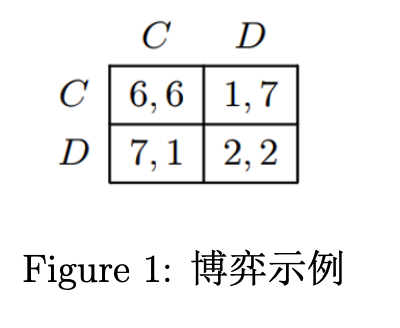
\includegraphics[width=0.25\textwidth]{./figure/fig1.png}
\end{figure}

\begin{problem}
	判断题:Figure-1博弈中纯策略组合$(C,D)$为帕雷托最优。
	\solution 是。在帕累托最优的条件下,是没有办法在不让某一参与资源分配的一方利益受损的情况下,令另一方获得更大利益的。
\end{problem}

\begin{problem}
	判断题:Figure-1博弈中纯策略组合$(C,D)$为纳什均衡。
	\solution 否。纳什均衡:没有参与者可以透过改变自身策略使自身受益时的一个概念解。
\end{problem}

\begin{figure}[htbp]
	\centering\label{fig:2}
	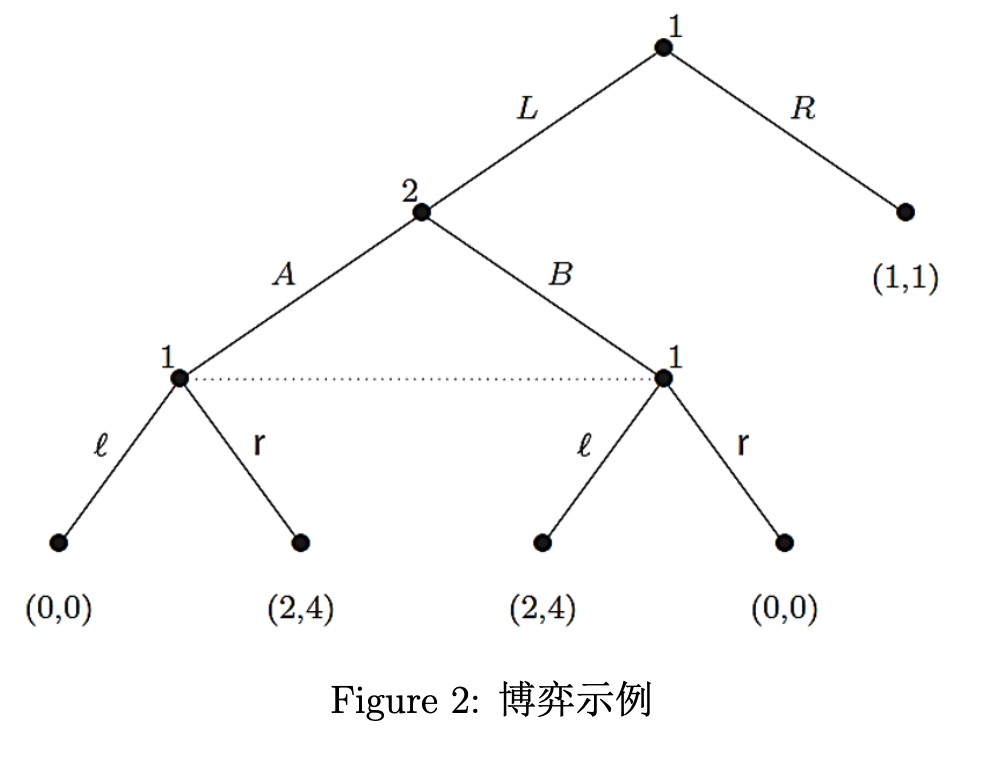
\includegraphics[width=0.6\textwidth]{./figure/fig2.png}
\end{figure}

\begin{problem}
	解释:Figure-2博弈中虚线的含义。
	\solution 虚线将属于同一信息集的所有决策结连接起来。此时决策者不知道自己处于哪一个点,可能处于虚线连接的任何一个点。
\end{problem}

\begin{figure}[htbp]
	\centering\label{fig:3}
	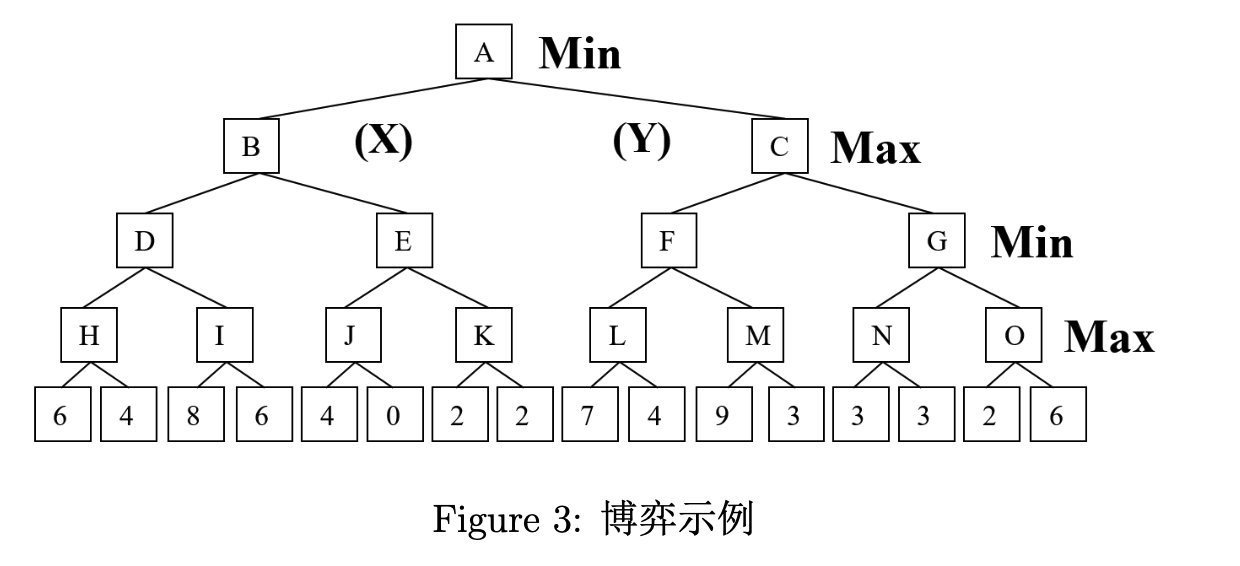
\includegraphics[width=0.8\textwidth]{./figure/fig3.png}
\end{figure}

\begin{problem}
	利用Minimax搜索算法判断Figure-3博弈中Min的最优初始选择是$X$还是$Y$?
	\solution 选择X。
\end{problem}

\begin{problem}
	利用$\alpha-\beta$剪枝算法判断Figure-3博弈中哪条枝可以剪掉。(至少写出两条枝,一条枝可以写成例如$A-B$或$H-6$的形式)。
	\solution $I-6, E-K, M-3, L-4, C-G$
\end{problem}

\begin{problem}	
	三羊问题。在你眼前有$3$扇巨大的关闭的门,编号分别是A、B、C。站在旁边的主持人告诉你,其中一扇门的后面摆着极为诱人的大奖(比如说一辆小轿车),而另外两扇门的后面各站着一头羊,你需要在这3扇门中选择1扇门,并获得那扇门后面的奖品。你经过深思熟虑,选择了编号为A的门,在你紧张兮兮正准备打开时,通晓一切的主持人说慢着,然后他打开了编号为C的门,后面正好是一头山羊,然后他问你:现在再给你一次选择的机会,你是坚持选择现在的门A,还是更换成门B?给出你的理由。
	\solution 问题的答案是可以:当参赛者转向另一扇门而不是维持原先的选择时,赢得汽车的机会将会加倍。
	有三种可能的情况,全部都有相等的可能性(1/3):
	\begin{itemize}
		\item 参赛者挑山羊一号,主持人挑山羊二号。转换将赢得汽车。
		\item 参赛者挑山羊二号,主持人挑山羊一号。转换将赢得汽车。
		\item 参赛者挑汽车,主持人挑羊一号。转换将失败。参赛者挑汽车,主持人挑羊二号。转换将失败。
	\end{itemize}
\end{problem}

\end{document}